\chapter{Supergravity }\label{ch:supergravity}


Quantum gravity theories must contain massless spin 2 particles, that are gravitons.
In the same fashion as we built super-Yang-Mills (SYM) theories, with maximum spin 1,
we can build supergravity (SUGRA) theories by requiring the supermultiplet to contain gravitons (and no higher spin particles).
This constrains the number of super-Poincar\'e charges to a maximum of 32\footnote{
In the unitary massless spinor representation $S$, half of the supercharges annihilates the highest weight state.
Only half of the remaining supercharges are spin-raising operators (the other half lowers spin).
On the hand, we can have at most 8 raising operators from spin -2 to 2 by steps of 1/2. 
Then (see e.g. \cite{DHoker:2002nbb}), for $\mathcal{N}$ copies of supersymmetries:
\[
1/4 \times \mathcal{N} \times \text{dim } S = 8 
\quad \Rightarrow \quad
\mathcal{N}  \text{dim } S = 32.
\]
}.


For one copy of supersymmetry, i.e. $\mathcal{N} = 1$, 
we have a unique supergravity theory in 11 dimensions \cite{Cremmer:1978km}, 
from which many lower dimensional supergravity theories can be obtained by the means of 
Kaluza-Klein compactication and dimensional reduction.
This theory contains a metric, an antisymmetric rank 3 tensor and a Majorana gravitino field.


Compactifying it on a circle and taking its radius to be zero, 
we obtain type IIA $\mathcal{N}=2$ SUGRA in 10 dimensions,
which is also a low energy effective action of type IIA superstring theory.
Using T-duality\footnote{
It states that strings compactified on a torus with radius $R$ is equivalent to strings compactified on a torus with
radius proportional to $1/R$.}, 
we can obtain type IIB $\mathcal{N}=2$ SUGRA,
% which is chiral (i.e. violates parity).
which is of our interest to study the AdS/CFT duality.
Let us list its field content:
\begin{center}
 \begin{tabular}{ |l | l| }
  \hline
  rank 2 symmetric tensor: metric & $g$ \\  \hline
  complex scalar: axion-dilaton  & $C_{(0)} + i \,e^{-\Phi}$ \\ \hline
  rank 2 antisymmetric tensor & $C_{(2)} + i \, B_{(2)}$ \\ \hline
  rank 4 antisymmetric tensor & $C_{(4)}$\\\hline
  Majorana-Weyl $3/2$-spinor: gravitinos & $\psi_M^I, \: I=1,2 $\\\hline
  Majorana-Weyl $1/2$-spinor: dilatinos & $\lambda^I, \: I=1,2 $ \\\hline
\end{tabular}
\end{center}
The gauge potentials $C_{(i)}$ are called the Ramond-Ramond potentials.
% The theory does not have a manifestly Lorentz-invariant action principle, it does have covariant field equations.
The fields above must satisfy the supergravity equations that consist of \cite{Schwarz:1983qr}:
\begin{itemize}
 \item Einstein's equations
 \item Maxwell's equations
 \item The dilaton equation
 \item (Hodge) self-duality equation: $*F_{(5)} = F_{(5)}$,  where \\
	\begin{equation} \label{5form}
	 F_{(5)} = dC_{(4)} - \dfrac{1}{2} C_{(2)}\wedge dB_{(2)} + \dfrac{1}{2} B_{(2)} \wedge dC_{(2)}.
	\end{equation}
\end{itemize}
To avoid introducing more notation, we refer the reader to e.g. \cite{Buchel:2000cn} 
for explicit expressions of the above equations.

The supersymmetry condition imposes the variation of dilatinos and of gravitinos to be zero \cite{Schwarz:1983qr}.
These are Killing equations and by solving them we obtain the Killing spinors of the background geometry.
For $AdS_5 \times S^5$, the solutions can be found in \cite{Skenderis:2002vf},
and for the Pilch-Warner background, see \cite{Pilch:2003jg} and the appendix D of Paper III.


\section{$AdS_5 \times S^5$}
The simplest solution to the supergravity equations is $AdS_5 \times S^5$ geometry,
where the dilaton $\Phi$, the $B$-field and the gauge potentials $C_{(0)}$ and $C_{(2)}$ are trivial.
% and it has the (Ramond-Ramond) 5-form flux \eqref{5form}.

Since spheres are more familiar, let us review only the metric of the anti-de-Sitter space ($AdS$).
It is a hyperboloid with Minkowski signature, embedded in the flat space of one dimension higher, i.e.:
% The Anti-de-Sitter spacetime of $D+1$-dimension ($AdS_{D+1}$) is a maximally symmetric solution of vacuum Einstein's equation with negative cosmological constant.
% In D+2 dimensions with signature $(-,-,+,\ldots,+)$, it is naturally embedded in the flat space 
\begin{equation}
 ds^2 = -dX_0^2-dX_D^2+\sum_{i=1}^{d-1} X_i^2
\end{equation}
with the constraint 
\begin{equation} \label{hyperboloid}
 - X_0^2 - X_d^2 + \sum_{i=1}^{d-1} X_i^2 = - L^2.
\end{equation}
Figure \ref{fig:AdS} shows an example for $AdS_2$.
The isometry group is clearly $SO(2,d)$.

By solving the constraint, the induced metric (in global coordinates) for $AdS_{d+1}$ becomes:
\begin{equation}
 ds^2 = L^2(-\cosh^2 \rho d\tau^2 + d\rho^2+\sinh^2\rho d\Omega_{d-1}^2).
\end{equation}
where $d\Omega_{d}^2$ is the metric of $S^d$, $\rho\geq 0$ and $2\pi \geq \tau \geq 0$.

Another set of solutions that solve the constraint \eqref{hyperboloid} is the Poincar\'e coordinates.
These are preferred for holographic studies, 
since the metric in these coordinates 
\begin{equation}\label{metricAdS}
 ds^2 = \dfrac{L^2}{z^2} (\eta_{\mu\nu} dx^\mu dx^\nu+dz^2 ) 
\end{equation}
is manifestly conformal invariant, with flat space slicing for any $z>0$ (see figure \ref{fig:AdS}), 
despite it covers only half of the geometry.
% The metric for $AdS_5\times S^5$ in the Poincar\'e patch is:
% \begin{equation}\label{metricAdS5S5}
%  ds^2_{AdS_5\times S^5} = \dfrac{L^2}{z^2} (-dt^2+d\mathbf{x}^2+dz^2 ) + L^2 d\Omega_5.
% \end{equation}
The conformal boundary\footnote{
The boundary of $AdS$ is infinitely far aways from the bulk,
but it can be mapped to a finite distance using a conformal transformation.} 
corresponds to $z \rightarrow 0$, 
and $z$, called radial coordinate, is interpreted as the energy scale of the boundary theory in AdS/CFT.
% This statement is made more clear using holographic renormalization, see e.g. the lectures \cite{Skenderis:2002wp}.

\begin{figure}[t]
\begin{center}
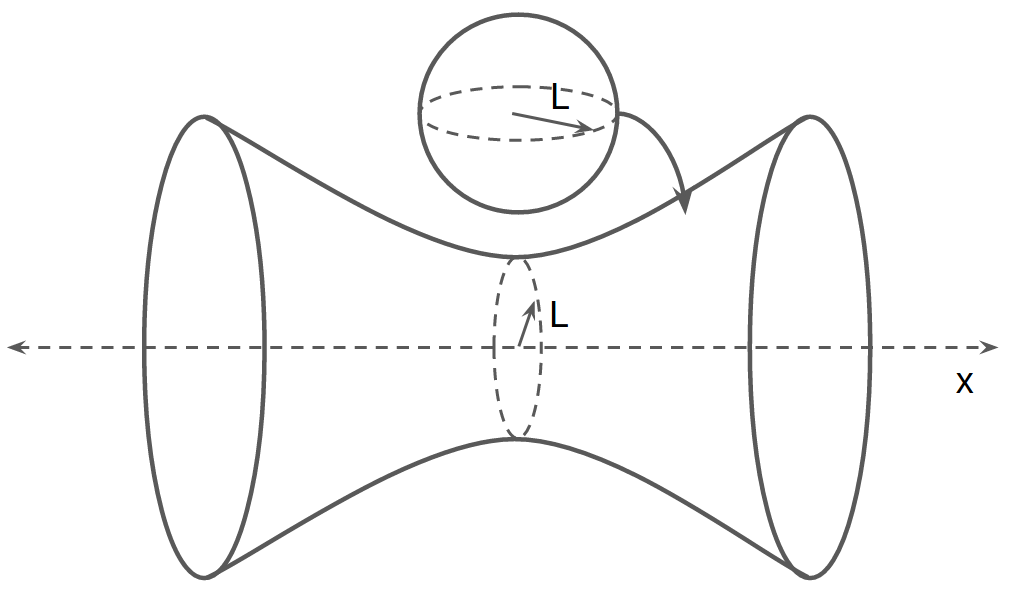
\includegraphics[width=0.49\textwidth]{Images/AdS2xS2.png}
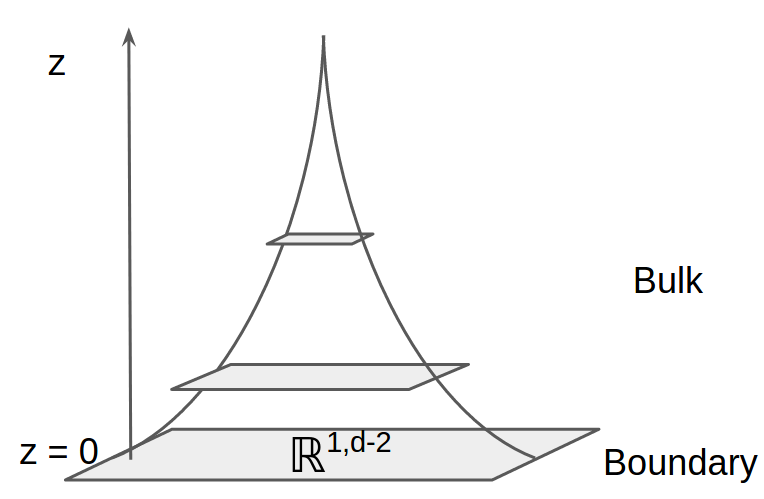
\includegraphics[width=0.49\textwidth]{Images/AdSPoincare.png}
\end{center}
\caption{\label{fig:AdS} Left: $AdS_2\times S^2$, where $AdS_2$ is defined by $x^2-y^2-t^2 = - L^2$, 
and at all its surface points we find the sphere.
Right: Flat space slicing for $AdS_d$ in Poincar\'e coordinates.}
\end{figure}

\section{D-branes}

D-branes are soliton-like solutions of the supergravity equations 
that preserve half of the 32 background supercharges (BPS solutions), see textbook \cite{Ammon:2015wua}:
\begin{eqnarray}
 ds^2   &=& H_p(r)^{-1/2} \eta_{\mu\nu}dx^\mu dx^\nu +  H_p(r)^{1/2} \delta_{ij} dy^i dy^j\\
 e^\Phi &=& g_s H_p(r)^{(3-p)/4}\\
 C_{(p+1)}&=&(H_p(r)^{-1} - 1) dx^0\wedge\cdots\wedge dx^p\\
 B_{(2)} &=& 0,
\end{eqnarray}
where $x^\mu, \mu=1,\ldots, p$ are the D-brane worldvolume coordinates, 
$y^i, i=p+1,\ldots,9$ are the transversal directions to the brane,
and the harmonic function is
\begin{equation}
 H_p(r) = 1 + \left( \dfrac{L_p}{r}\right)^{7-p}.
\end{equation}

It is intuitive to think of these solutions as charged point-like particles from the $(9-p)$-dimensional transverse space point of view.
For $N$ coincident D-branes, their total charge is proportional to $N$,
and from the Gauss law, we obtain
\begin{equation}
 N \propto \int_{S^{9-p-1}} *F_{(p+2)},
\end{equation}
quantizing therefore the (Hodge dual) of the flux of the Ramond-Ramond field $C_{(p+1)}$ through the hypersphere, $F_{(p+2)}$.
The above relation also determines the characteristic length scale 
\begin{equation}\label{characteristicLengthLp}
 L_p^{7-p} = (4\pi)^{(5-p)/2} \Gamma \left(\dfrac{7-p}{2}\right) g_s N \alpha'^{(1-p)/2},
\end{equation}
where $g_s$ is the string length and $\alpha'$ is the Regge slope. 
We will comment on these parameters in chapter \ref{chp:AdSCFT},
where we will also see that $AdS_5 \times S^5$ geometry can be obtained as the near horizon geometry of a stack of $N$ coincident D3-branes.

To conclude this section, 
let us write down the generic action of a single D-brane in Minkowski signature, 
which will be used later on in the thesis.
The action consists of the Dirac-Born-Infeld (DBI) term:
\begin{equation}\label{DBI}
 S_\text{DBI} = -T_\text{Dp} \int_M\,  d^{p+1}\xi e^{-\Phi} \, \sqrt{-\text{det}\left( P[g] + P[B] + \dfrac{1}{T_\text{F1}} F \right)},
%  d^{p+1}\sigma \,
\end{equation}
and the Wess-Zumino (WZ) term with the Ramond-Ramond potentials pulled back to the worldvolume:
\begin{equation}\label{WZ}
 S_\text{WZ} = T_\text{Dp} \int_M\, \exp{\left(P[B] + \dfrac{1}{T_\text{F1}} F \right)} \wedge  P[C].
\end{equation}
The couplings are
\begin{equation} \label{couplingsTension}
 T_\text{F1} = \dfrac{1}{2\pi\alpha'},
 \quad 
 T_\text{D1} = \dfrac{1}{g_s}\,T_\text{F1},
 \quad 
 T_\text{Dp} =  T_\text{D1}\left(2\pi \sqrt{\alpha'}\right)^{1-p}.
\end{equation}
% and we use the replacement rules $\alpha'\rightarrow 1/\sqrt{\lambda}$ and $g_s \rightarrow \lambda/(4\pi N)$ 


\section{Pilch-Warner geometry}
Another solution that preserves $\mathcal{N}=2$ supersymmetric flow is found by Pilch-Warner \cite{Pilch:2000ue}.
The geometry is a deformed and warped $AdS_5 \times S^5$, and all the fields are non-trivial in this case.
The metric (in Einstein frame) is
% \footnote{
% The string metric $g$ and the Einstein metric $G$ are related by $g=e^{-\frac{4 \Phi }{D-2}} G$,
% where $\Phi$ is the dilaton.
% }
\begin{eqnarray}\label{metricPW}
 ds^2 & = & \dfrac{(c \, X_1 X_2)^{1/4}}{\sqrt{A}} L^2
	\left( 
	  \dfrac{M^2 A}{c^2-1} \eta_{\mu\nu}dx^\mu dx^\nu + \dfrac{1}{A (c^2-1)^2} dc^2 
	\right.\\
      & & +\left. \left[
		  \dfrac{1}{c} d\theta^2 + \dfrac{\sin^2\theta}{X_2} d\phi^2 
		  + \cos^2\theta  \left(\dfrac{A}{X_1}(\sigma_1^2 +\sigma_2^2) + \dfrac{A}{c \, X_2} \sigma_3 \right)  
		\right] 
        \right),\nonumber
\end{eqnarray}
where $\sigma_i, i=1,2,3$ are the Maurer-Cartan forms for $SU(2)$ and
\begin{eqnarray*}
 & X_1(c,\theta) =  \cos^2\theta + c\, A(c)  \sin^2\theta, \\
 &  X_2 (c,\theta)=  c \cos^2\theta + A(c)  \sin^2\theta, \\
 & A(c)  = c+\dfrac{1}{2}(c^2 - 1)\log\left(\dfrac{c-1}{c+1}\right).
\end{eqnarray*}
It reduces to $AdS_5 \times S^5$ near the boundary, i.e. expand the metric for $c \approx 1 + z^2 M^2/ 2$, 
where $z$ is the radial coordinate in \eqref{metricAdS}, then set $M=0$.

The Pilch-Warner solution is dual to $\mathcal{N}=2^*$ SYM on $\mathbb{R}^4$. 
% It is obtained using holographic renormalization for a truncated $\mathcal{N} = 8$ 5-dimensional SUGRA.
% That is, imposing supersymmetric  an asymptotic $AdS_5$ metric ansatz  and then lifted to 10d supergravity. 
Similarly the dual for $\mathcal{N}=2^*$ on $S^4$ has been studied in \cite{Bobev:2013cja},
but the solution is partially known only.
We are interested in the flat space regime, where interesting physics happen such as the phase-transitions discussed in Part I (see figure \ref{fig:phaseDiagram}).
Hence, the dual computations will be done in the Pilch-Warner background.





% \section{AdS geometry}
% 
% The Anti-de-Sitter spacetime of $D+1$-dimension ($AdS_{D+1}$) is a maximally symmetric solution of vacuum Einstein's equation with negative cosmological constant.
% In D+2 dimensions with signature $(-,-,+,\ldots,+)$, it is naturally embedded in the flat space 
% \begin{equation}
%  ds^2 = -dX_0^2-dX_D^2+\sum_{i=1}^{D-1} X_i^2
% \end{equation}
% with the constraint 
% \begin{equation}
%  - X_0^2 - X_D^2 + \sum_{i=1}^{D-1} X_i^2 = - l^2.
% \end{equation}
% The isometry group is $SO(2,d)$
% If the D dimension were Euclidean, the previous equation is a two-sheeted hyperboloid.
% (figures)
% 
% The constraint is solved by
% \begin{equation}
%  X_0 = l \cosh \rho \cos \tau , \quad 
%  X_D = l \cosh \rho \sin \tau , \quad 
%  X_i=l \eta_i \sinh \rho
% \end{equation}
% where the angles $\eta_i$ are such that $\sum_{i=1}^{D-1} \eta_i = 1$, 
% and $\rho\geq 0$ and $2\pi \geq \tau \geq 0$.
% \begin{equation}
%  ds^2 = l^2(-\cosh^2 \rho d\tau^2 + d\rho^2+\sinh^2\rho d\Omega_{d-1}^2).
% \end{equation}
% These new parameters form the global coordinates of AdS, since they cover the full hyperboloid.
% 
% There is another set of solutions that cover only half of the hyperboloid:
% \begin{eqnarray}
%  X_0 &=& \dfrac{1}{2}(z+\dfrac{1}{z}(l^2+\mathbf{x}^2 - t^2))\\
%  X_D &=& \dfrac{1}{2}(z-\dfrac{1}{z}(l^2-\mathbf{x}^2 + t^2))\\
%  X_1 &=& \dfrac{l}{z} t\\
%  X_i &=& \dfrac{l}{z} r
% \end{eqnarray}
% We call the above solution the Poincar\'e patch, and the metric is
% \begin{equation}
%  ds^2 = \dfrac{l^2}{z^2} (-dt^2+d\mathbf{x}^2+dz^2 )
% \end{equation}
% This form is manifestly conformal invariant, and is very useful for holographic computations.
% The conformal boundary corresponds to $z \rightarrow 0$.
% 
% % spherical geometry?
% % 
% % Killing spinor?






  
